%----------------------------------------------------------------------------------------
%	SOLUTION 3.1
%----------------------------------------------------------------------------------------
\subsection*{Problem 3.1}
Absolute value of the slope of I-V curve near the open circuit voltage is approximately equal to $\frac{1}{R_s}$. From the given graph, we can calculate the slope and find
\begin{align*}
	& \frac{1}{R_s} = \frac{1.4-1.0}{0.58-0.56}\\
	\implies & R_s = 0.05\ \Omega.
\end{align*}
%----------------------------------------------------------------------------------------
%	SOLUTION 3.2
%----------------------------------------------------------------------------------------
\subsection*{Problem 3.2}
The absolute value of the slope of I-V curve near the short circuit current is approximately equal to $\frac{1}{R_p}$. From the given graph,
\begin{align*}
	& \frac{1}{R_p} = 0\\
	\implies & R_p = \infty\ \Omega.
\end{align*}
%----------------------------------------------------------------------------------------
%	SOLUTION 3.3
%----------------------------------------------------------------------------------------
\subsection*{Problem 3.3}
From the graph, approximately it looks maximum power point, for the curve labeled as $R_s=0$ is near $V=0.56$ V and $I=3.8$ A. Therefore, the maximum power that can be delivered is $P_{max} = (0.56)(3.8) = 2.13$ W.
%----------------------------------------------------------------------------------------
%	SOLUTION 3.4
%----------------------------------------------------------------------------------------
\subsection*{Problem 3.4}
In case of $5$ parallel strings of $10$ series connected cells, the open circuit voltage would be $0.63\times 10 = 6.3$ V and short circuit current would be $4\times 5 = 20$ A. As for the curve labeled with $R_s=0$ is having approximately very large parallel resistance ($R_p \leftarrow \infty$), as estimated before, and series resistance $R_s=0\ \Omega$, as indicated in the given graph. Therefore, we can assume that there will not be significant effect on the slope of the I-V curve near open circuit as well as short circuit condition. An approximate I-V curve for the series-parallel combination is shown in Fig.~\ref{fig:q3_4_iv_curve}.
\begin{figure}[h]
	\centering
	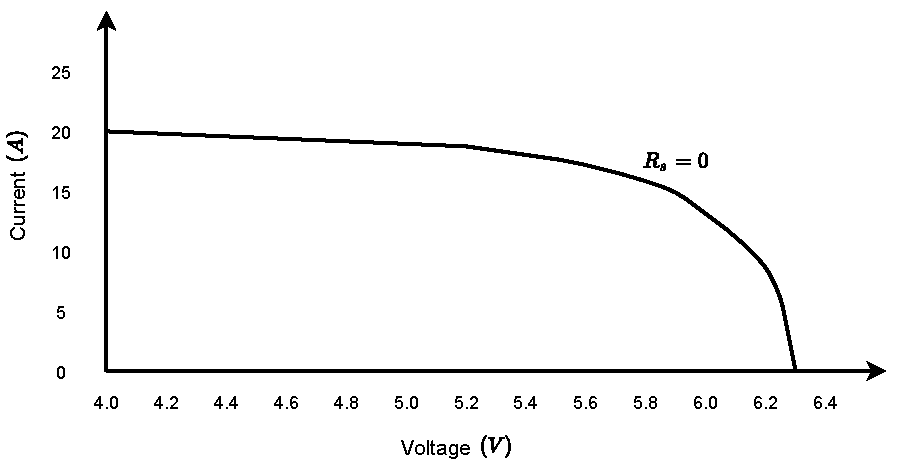
\includegraphics[scale=1.0,trim={0cm 0cm 0cm 0cm},clip]{./q3_4_iv_curve.pdf}
	\caption{I-V curve of $5$ parallel strings each with $10$ series-connected PV cells}
	\label{fig:q3_4_iv_curve}
\end{figure}